\section{Transformadas de Fourier Famosas}

Uma transformada pega numa função (ou sinal) e transforma-a numa outra função (ou sinal).
A transformada discreta de Fourier é dada pela seguinte expressão:
\begin{equation}
    H(f)=\int_{-\infty}^{+\infty} h(t)\cdot e^{2\pi ift} \cdot dt 
\end{equation}

A transformada rápida de Fourier (do inglês: \emph{Fast Fourier Transform}, abreviado FFT), é um algoritmo que calcula a transformada discreta de Fourier. A análise de Fourier converte um sinal do domínio original (tempo) para uma representação no domínio das frequências e vice-versa.

\subsection{Função Seno \boldmath{$\rightarrow$} Função Delta} 

A transformada de Fourier de uma função sinusoidal é uma função delta de Dirac, pelo menos em parte. Quando aplicamos a transformada de Fourier no MATLAB (função \emph{fft}) a uma função sinusoidal, o resultado é uma combinação de deltas de Dirac localizados nas frequências da função sinusoidal. A transformada de Fourier da função é zero em todas as frequências exceto na frequência da função seno, onde há um Dirac localizado.

\lstinputlisting[style=Matlab-editor, basicstyle=\small, caption={Slide 12.}, label={lst: seno_delta}, firstline=2]{./codigo/seno_delta.m}

\newpage

É possível verificar pelos gráficos produzidos pelo código anterior, que o Dirac ocorre na frequência $7.98403\approx 8$, que é a frequência da função sinusoidal.

\begin{figure}[!ht]
    \centering
    \begin{minipage}[b]{0.49\textwidth}
        \centering
        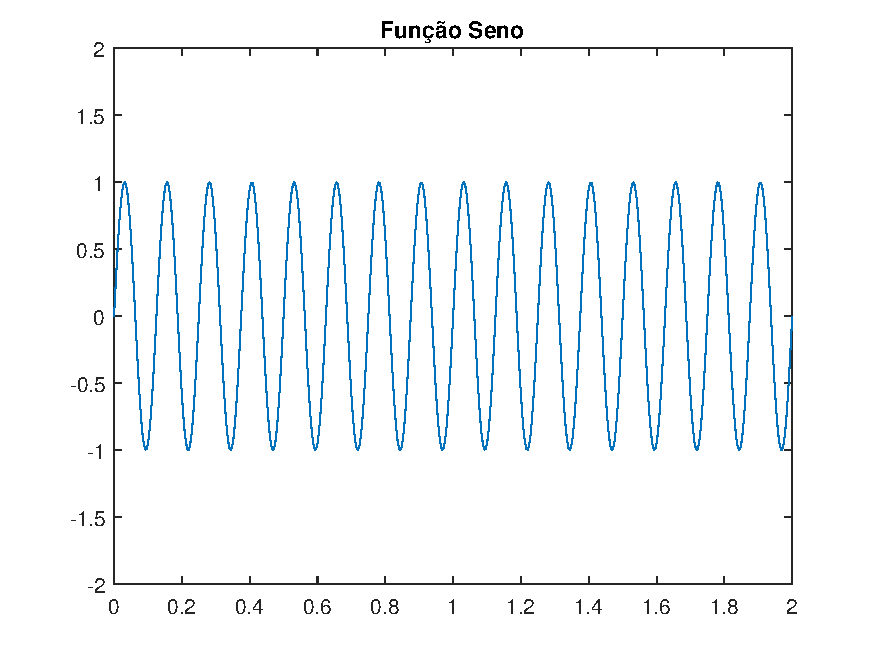
\includegraphics[width=\textwidth]{função seno.pdf}
        \caption{Função Seno.}
    \end{minipage}
    \hfill
    \begin{minipage}[b]{0.49\textwidth}
        \centering
        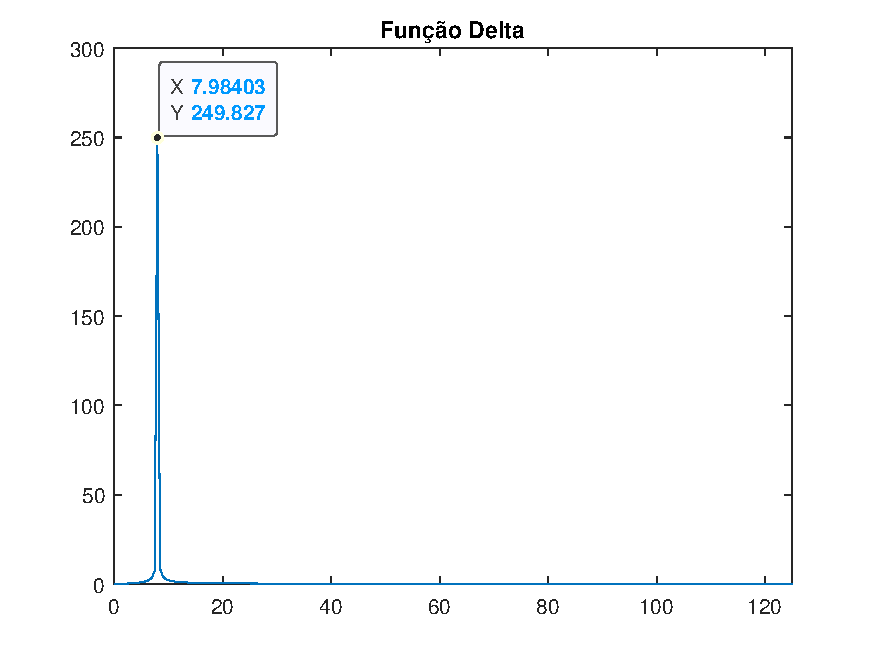
\includegraphics[width=\textwidth]{função delta.pdf}
        \caption{Função Delta.}
    \end{minipage}
\end{figure}

\subsection{Função Gaussiana}

A transformada de Fourier de uma função gaussiana é também uma função gaussiana mas com parâmetros diferentes.

\lstinputlisting[style=Matlab-editor, basicstyle=\small, caption={Slide 13.}, label={lst: gauss}, firstline=2]{./codigo/gauss.m}

Neste caso, a amplitude da transformada de Fourier é 5 e a média é 125. As figuras da página seguinte mostram a resposta do código apresentado.

\newpage

\begin{figure}[!ht]
    \centering
    \begin{minipage}[b]{0.49\textwidth}
        \centering
        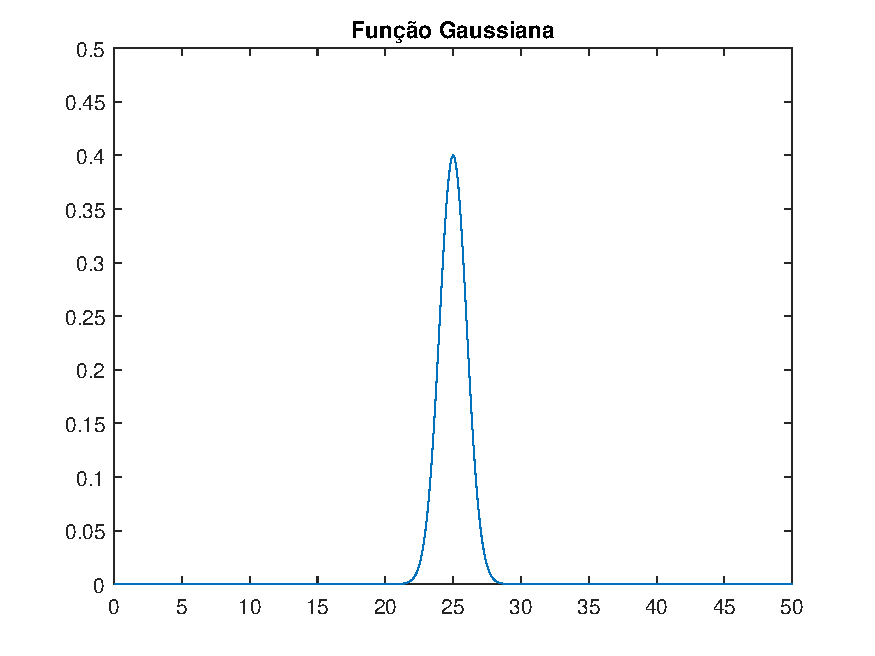
\includegraphics[width=\textwidth]{gauss.pdf}
    \end{minipage}
    \hfill
    \begin{minipage}[b]{0.49\textwidth}
        \centering
        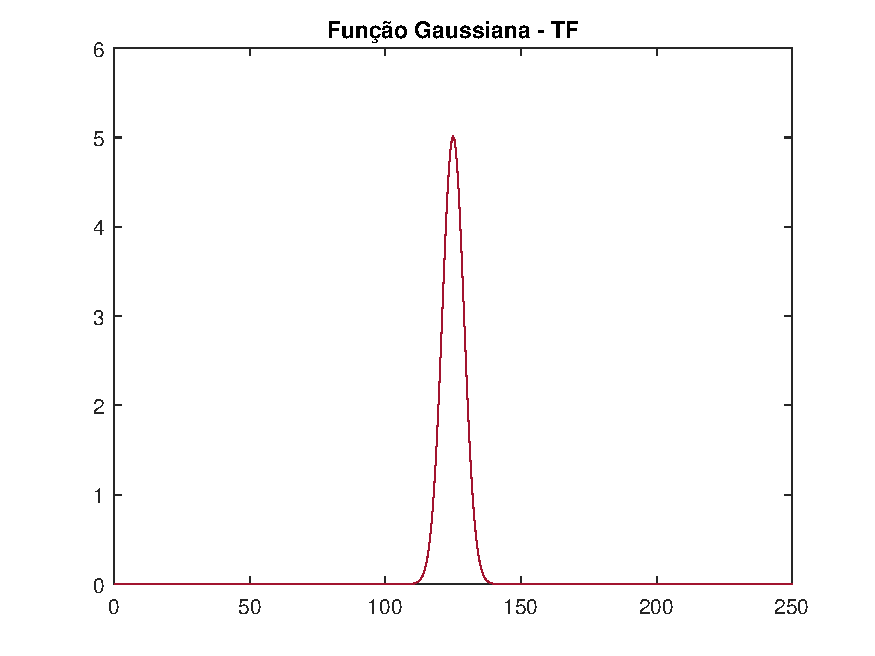
\includegraphics[width=\textwidth]{gaussTF.pdf}
    \end{minipage}
    \caption{Função Gaussiana e a sua transformada de Fourier.}
\end{figure}

\subsection{Função Seno Cardinal \boldmath{$\rightarrow$} \emph{Square Wave}}

\lstinputlisting[style=Matlab-editor, basicstyle=\small, caption={Slides 14 e 15.}, label={lst: sinc_ped}, firstline=2]{./codigo/sinc_ped.m}

A transformada de Fourier da função seno cardinal (sinc) resulta numa \emph{square wave} (pedestal). 

De forma intuitiva, a função seno cardinal tem oscilações até ao infinito e quando a sua transformada de Fourier é calculada, envolve a soma de componentes sinusoidais infinitas, o que resulta numa onda quadrada. 

Essencialmente, a transformada de Fourier da função seno cardinal capta a propriedade fundamental desta função, nomeadamente o seu comportamento oscilatório, que no eixo das frequências, resulta numa \emph{square wave}.

\begin{figure}[!ht]
\centering
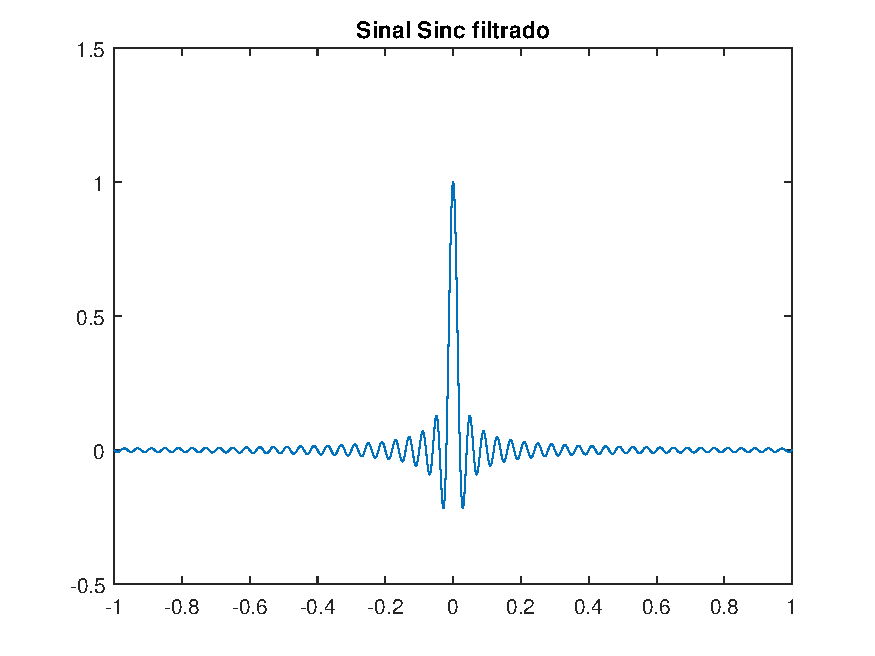
\includegraphics[width=0.75\textwidth]{sinc.pdf}
\caption{Função Sinc.}
\end{figure}

\begin{figure}[!ht]
    \centering
    \begin{minipage}[b]{0.49\textwidth}
        \centering
        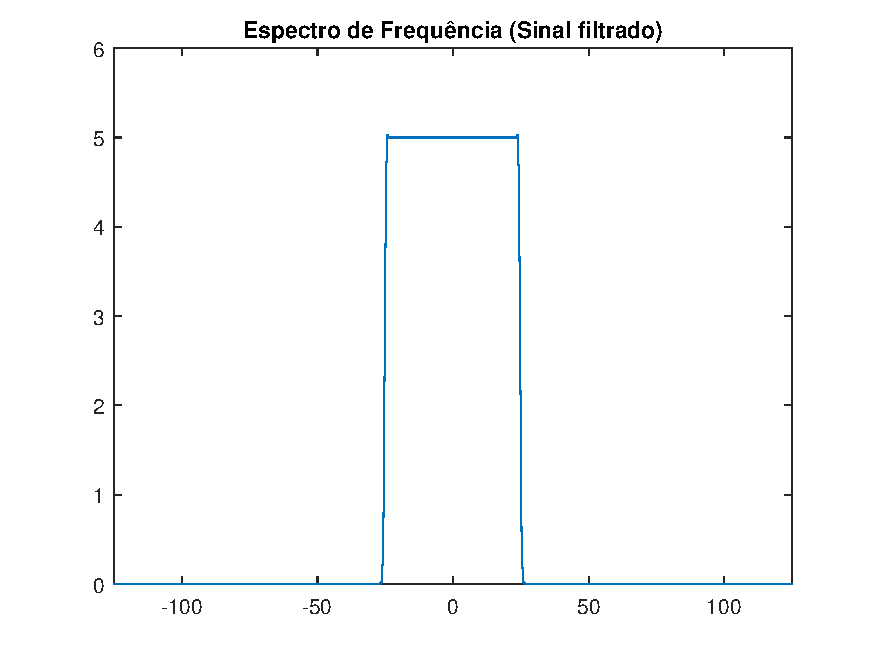
\includegraphics[width=\textwidth]{sinc2.pdf}
        \caption{Espectro de Frequências.}
    \end{minipage}
    \hfill
    \begin{minipage}[b]{0.49\textwidth}
        \centering
        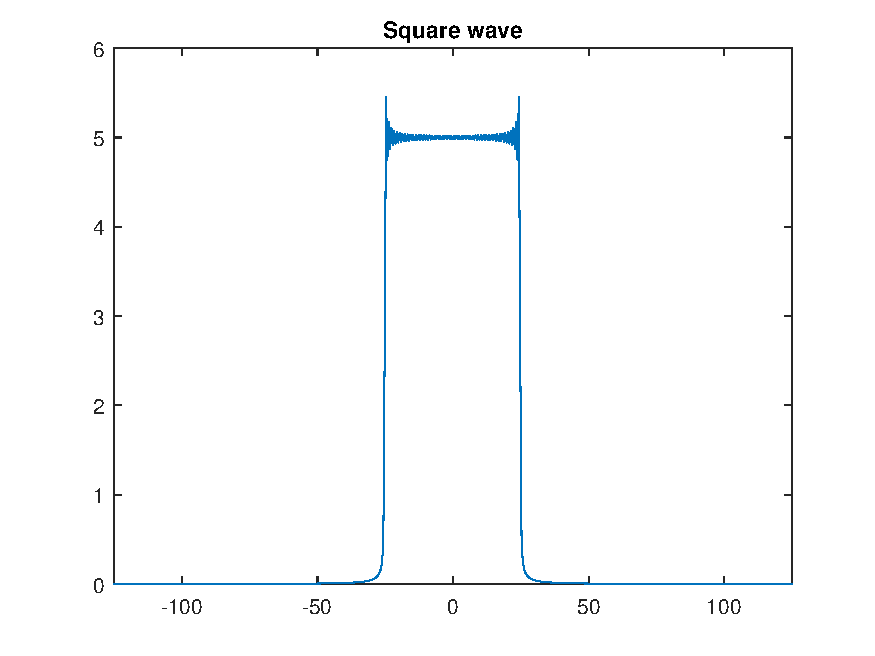
\includegraphics[width=\textwidth]{sinc3.pdf}
        \caption{Square Wave.}
    \end{minipage}
\end{figure}

\newpage

\subsection{Função Exponencial \boldmath{$\rightarrow$} Lorentziana}

\lstinputlisting[style=Matlab-editor, basicstyle=\small, caption={Slide 16.}, label={lst: exp_lorentz}, firstline=2]{./codigo/exp_lorentz.m}

\begin{figure}[!ht]
    \centering
    \begin{minipage}[b]{0.49\textwidth}
        \centering
        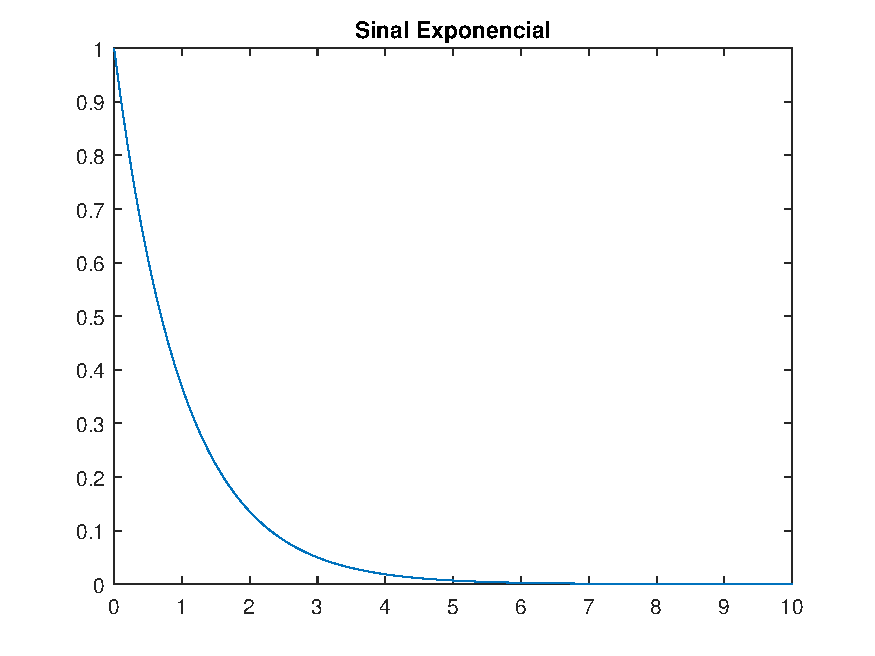
\includegraphics[width=\textwidth]{exp_lorentz1.pdf}
        \caption{Função Exponencial.}
    \end{minipage}
    \hfill
    \begin{minipage}[b]{0.49\textwidth}
        \centering
        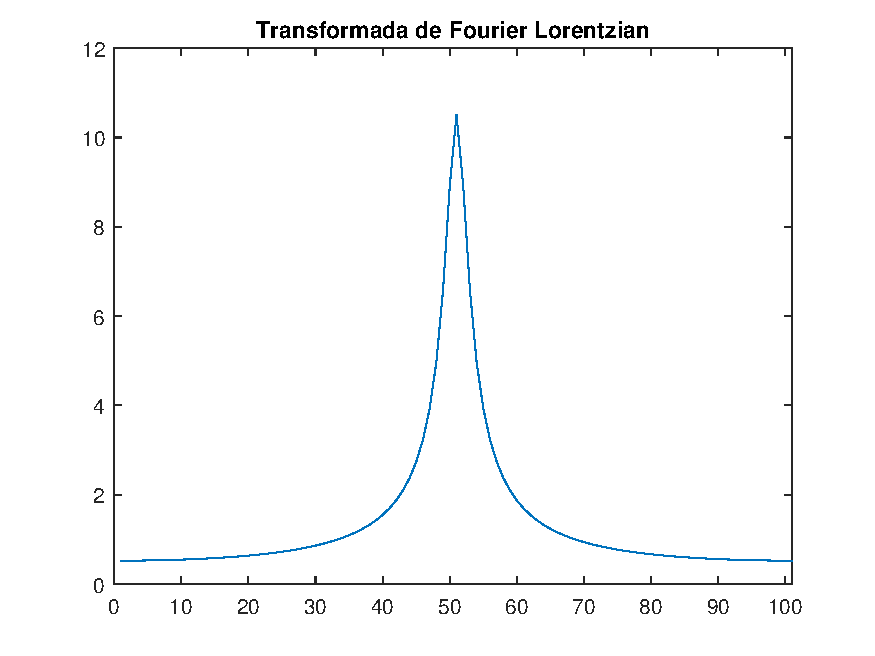
\includegraphics[width=\textwidth]{exp_lorentz2.pdf}
        \caption{Função Lorentziana.}
    \end{minipage}
\end{figure}